\documentclass{jdrp}

\bibliography{tex/references} 

\newcommand*{\crg}{{\aurebesh\Large \$}} % Symbol for Galactic Credits

\hypersetup{  
  pdfinfo={  
    Title={SWR - La Citadelle Hurlante},
    Subject={Scénario, Citadelle Hurlante},
    Author={Marthym},
    Keywords={starwars,savage,worlds,jdr,scenario},  
    Copyright={Do What The Fuck You Want To Public License}
  }  
} 

\begin{document}

	\begin{titlepage}

	\begin{center}
		\hspace*{\vfill}
		\noindent\Huge\jedifont{Star Wars Redemption}\\ 
		\noindent\fontsize{50}{70}\jedifont{\$}
		\noindent\fontsize{50}{70}\jedifont{\#}\\
		\noindent\fontsize{50}{60}\jedifont{La Citadelle Hurlante}
		\hspace*{\vfill}
	\end{center}

	%\hspace*{\vfill}

	\noindent\makebox[\textwidth]{
		\includegraphics[width=\paperwidth]{swr-class/_img/cover-bg.png}}
	\begin{tikzpicture}[overlay]
		\node[minimum width=200pt,minimum height=200pt, rotate=0] at (2,5){\includegraphics[width=200pt]{_img/places/citadel-of-ktath-atn.png}};
	\end{tikzpicture}}
	\end{titlepage}

	\onecolumn
	\section{avant propos}
	
	\begin{wrapfigure}{R}{180pt}
		\centering
		
\includegraphics[width=180pt]{_img/pnjs/aphra.png}
		\caption{\label{fig:aphra}Docteur Aphra}
		\vspace{1\baselineskip}
		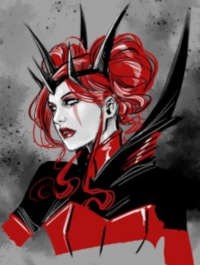
\includegraphics[width=180pt]{_img/pnjs/ktath-atn-queen.png}
		\caption{\label{fig:ktath-atn-queen}Reine de Ktath’Atn}
	\end{wrapfigure}

	Ce scénario est pleinement inspiré du spin-off entre la série \citetitle{starwars-marvel} & \citetitle{starwars-aphra}. Il est initialement prévue pour être joué selon les règles des \citetitle{jdrp-starwars}. Le scénario est écrit pour une petite équipe de héros (3 à 5) déjà formé mais la première scène peu être facilement adapté. Un padawan ou un Jedi est nécessaire, si votre équipe n’en contient pas, il faudra soit adapter le scénario pour l’un de vos joueurs, soit ajouter un PNJ padawan.

    \bigbreak
    
    Le scénario se passe peu après la destruction de la première Etoile de la mort par le jeune Luke Skywalker. Vos héros se trouvent embarqués par le Doctor Aphra, archéologue un peu frappée à la morale douteuse. Cette dernière a besoin d’une forme de vie organique "intéressante" à présenter à la reine de la Citadelle Hurlante pour accéder à la mémoire d’un ancien Jedi. Aucun padawan ne peu refuser une offre pareille...

    \bigbreak

    Ce scénario est initialement pensé pour des héros tendant vers le coté lumineux de la Force mais je proposerais chaque fois que nécessaire une version pour le coté obscur.

    \vspace*{\fill}

	\subsection{Licence}
	\noindent DO WHAT THE FUCK YOU WANT TO PUBLIC LICENSE\\
    Version 2, December 2004
    \vspace{-2.5\baselineskip}
	\begin{flushright}
		\includegraphics[width=70pt]{swr-class/_img/wtfpl-badge.png}
	\end{flushright}

	\twocolumn

	\section{Docteur Aphra}

\subsection{introduction}
Ce scénario commence dans une cantina pas vraiment accueillante d’Horox III. Les héros aspirent à un peu de repos bien mérité après une mission pour l’alliance qui n’a pas vraiment été une franc succèss.

Ils avaient pour objectif d’identifier l’origine d’un traffic de matrices droïde modifié pour le combat. Malheureusement après deux semaines de recherche et d’intérogatoire, tout ce qu’ils ont réussit c’est a se prendre une correction par l’un des fameux droïdes modifiés. 

\begin{paperbox}{Coté obscur}
Les héros étaient en mission pour l’empire. Il sont à la recherche de individu capable de modifier les matrices de droïde pour en faire des droïdes de combat plutôt performant. Le seigneur Vador se montre très intéressé car il souhaite se monter une armée personelle.
\end{paperbox}

\subsection{Viens voir le docteur}
Les voilà donc ruminant leur échec dans un bar quand entre une femme, brune, mince, un bonnet et de lunettes d’aviateur sur la tête. L’horoxien au bar lève la tête et semble, l’espace d’un instant surpris. Puis il se reprend et interpelle violament la femme :

\begin{quotebox}
- \textbf{barman} Aphra ! Tu ne manque pas d’aplomb de te repointer ici ! Les droïdes que tu m’a refilé, c’était de la merde. Ils ont pas tenu 10 minutes !\\
- \textbf{Aphra} En face de ta sale gueule ça m’étonne pas !\\
- \textbf{barman} Attrapez là, on va lui faire sa fête !
\end{quotebox}

Les \nameref{sec:horoxian-barfly}, jusqu’à lors calmes, occupés à leur consomatoins se lèvent et commencent à pousser les tables. L’ambiance devient très tendu, la bagarre est inévitable. 

Si vos joueurs ont un peu de jujotte, il comprennent qu’\nameref{sec:aphra} a quelque chose à voir avec les matrices modifiés qu’ils recherchent, ou qu’au moins elle peut les aider. S’ils ne comprennent pas incitz les à entrer dans la danse avec une bouteille perdu par exemple.

\subsection{Docteur et Queen}
    \section{la citadelle}

\includegraphics[width=200pt]{_img/places/citadel-of-ktath-atn.png}

\textbf{Ktath’Atn} est une planète peu accueillante, il y pleut presque tout le temps. L’Empire n’y a aucune prise, la reine y règne d’une main de fer, sans pitié ni compassion. Il lui arrive d’être manianime mais jamais sans raison. La \nameref{sec:ktath-atn-queen} est imprévisible et il ne faut pas la sous-estimer, sous ses aspects gracieux se cache une tigresse sans pitié.

\begin{paperbox}{Séquence Narrative}
Ici commence une section narrative, sans combat (normalement). A vous de mettre les joueurs dans l’ambiance, il sera possible d’utiliser des compétences de charisme et de persuasion. Cette séquence est longue à écrire et à lire mais ne devrait pas durer des heures à jouer.
\end{paperbox}

\subsection{L’accueil}

\begin{wrapfigure}{r}{0.3\linewidth}
    \vspace{-4\baselineskip}
    \centering\hspace*{-.99\columnsep}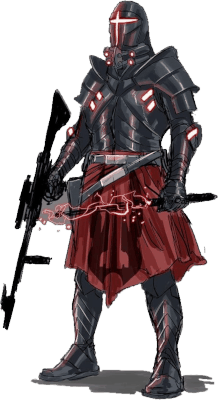
\includegraphics[width=1.2\linewidth]{_img/bestiary/citadel-guard.png}
    \vspace{-1\baselineskip} 
\end{wrapfigure}

A leur arrivé dans le périmêtre de Ktath’Atn, les héros et leur vaisseau sont dirigés vers une plateforme d’atterrissage où ils sont attendu par 4 \nameref{sec:citadel-guard} pour être escorté vers leurs quartiers avant la réception de ce soir.

L’un des gardes demande l’invitation, \nameref{sec:aphra} lui tend le document et les gardes font signe de les suivres. Ils encadrent le groupe ne laissant que peu de marge de manœuvre aux héros.

Les quartiers des invités se situent dans les premiers étages de la tour. Ce sont des appartements luxueux avec largement assez de place pour que chaque membre du groupe est de quoi poser ses affaires.

Le soir tombe sur la citadelle. Laissez les héros faire ce qu’ils souhaitent pour se préparer à la réception. Les blasters et les lames ne seront pas autorisés durant la soirée, une tenue correcte est de rigueur sous peine de perdre \textbf{-2 Cha}risme. 

\subsection{La réception}

Les héros débarquent dans une salle immense, style cathédrale, très haut de plafond, colonnes, \dots

A l’intérieur une centaine de personnes, de toutes espèce et de tous genre. Certains humanoïde, d’autres d’aspect gélatineux, mais tous organiques. Des droïdes font le service au milieu des invités. 

Si un ou plusieurs de vos héros sont des droïdes, ils ne se sentent pas à l’aise, ils perdent \textbf{-1 Cha}risme durant la soirée.

\begin{paperbox}{Mission bonus}
Plusieurs types d’interractions sont possible durant cette phase de la soirée. Un jet de \textbf{Pers}uasion \textbf{Diff}iculté \textbf{6} incitera les convives à parler à vos héros. Deux types d’informations sont alors disponibles, au MJ de distiller les infos selon ses préférences.

Les héros peuvent tenté d’en apprendre plus sur \nameref{sec:aphra}. S’ils posent la question aux bonnes personnes et que le jet est réussit, ils apprendront que \nameref{sec:aphra} n’est pas très fiable. Une partie des convives s’est déjà fait arnaqué par \nameref{sec:aphra} et serait ravi de lui rendre la pareille. Elle est clairement dans le commerce de droïdes de combat et en sait forcément plus que ce qu’elle a dit aux héros jusque là.

Les héros peuvent aussi apprendre ce que les autres invités ont prévu de présenter à la reine pour obtenir ses faveurs. Dans le tas, une sorte de fée clochette capable de répendre une poudre qui permet aux humanoïde de voler pendant une courte durée. Un guerrier Ezarien muni d’un exo-squelette naturel. Une sorte de taupe, capable de se téléporter sur courte distance quand elle éternue, \dots

Au MJ d’échanger avec les joueurs sachant que de toutes façons, la reine les choisira vos héros. 

Ce passage n’est pas obligatoire, si vos joueurs sont plus porté sur la castagne, ou si vous n’êtes pas un MJ aguerri à l’improvisation, ne vous lancez pas là dedans.
\end{paperbox}

Quand le MJ décide qu’il est temps (les joueurs n’interagissent pas/plus) c’est le moment de faire entrer la reine et ses sbires.\\

\noindent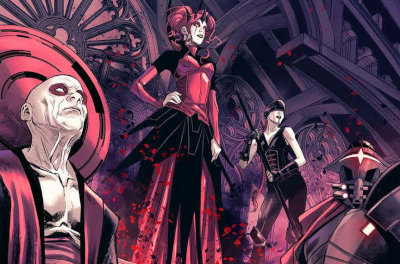
\includegraphics[width=\linewidth]{_img/places/queen-with-minions.jpg}

\begin{quotebox}
Bonsoir et merci à vous mes chers amis d’être venu ce soir, il me tarde de voir ce que vous avez à me présenter. Et comme promis celui qui me présentera la forme de vie organique la plus "intéressante" se vera accorder une de mes faveurs.

Mais ne trainons plus, commençons les présentations immédiatement.
\end{quotebox}

\nameref{sec:varroa} prend alors la parole et commence à appeler les invités un à un.

\begin{paperbox}{Présentations}
je ne décrit pas ici chaque présentation qui est faite. Je laisse au MJ le soin et l’imagination de faire passer des êtres plus ou moins étranges qui seront dignes ou non d’intéret. Quand les joueurs ont compris le principe, c’est à eux d’entrer en scène.
\end{paperbox}

\begin{quotebox}
\noindent\textbf{\nameref{sec:varroa}}: Docteur Aphra

\emph{\nameref{sec:aphra} fait signe aux héros de s’avancer avec elle.}

\noindent\textbf{\nameref{sec:varroa}}: Qu’avez vous a présenter à la reine.\\
\noindent\textbf{\nameref{sec:aphra}}: Un Jedi humain

\emph{Ou n’importe quoi selon les héros que vous avez.}
\end{quotebox}

A ces mots un silence assourdissant se fit entendre. Un guerrier Ezarien sort de la foule et prend \nameref{sec:aphra} à partie. Il est grand, fin et possède une sorte d’exo-squelette qui le protège des coups directs.

\begin{quotebox}
C’est un blague, les Jedis ont été éradiqués, qu’est ce que cet humain va pouvoir faire contre moi !
\end{quotebox}

Et le guerrier Ezarien se jette sur le Jedi. Vu que ce dernier a clairement montré ses intensions, la première attaque est pour le Jedi. L’enjeu ici est de faire une démonstration des pouvoirs à la reine. \'A la première utilisation visible des pouvoirs de Jedi, \nameref{sec:varroa} stoppe le combat. De son coté, le guerrier Ezarien n’a que ses poings.

Si par hasard le Jedi n’a pas accès à des pouvoirs visibles, laissez le se prendre quelques coups puis faites lui utiliser une \textbf{Poussée de Force} instinctive contre le guerrier. Cela suffira à impressionner la reine qui mettra fin au combat.

\begin{quotebox}
\noindent\textbf{\nameref{sec:varroa}}: La reine à choisie, tous les invités doivent partir immédiatement, la réception est terminée.

\emph{\nameref{sec:varroa} fait signe aux héros de s’avancer vers lui.}

\noindent\textbf{\nameref{sec:varroa}}: Ce soir nous vous offrons l’hospitalité. Demain vous déjeunerez avec la Reine, elle écoutera votre requête à ce moment. Allez dormir maintenant.
\end{quotebox}

Vos héros ont déjà pas mal bougé, ils vont se coucher. Pas d’exploration pour l’instant, on verra demain.

    \section{la dejeune}
	\section{Personnages}
Les personnages avec un ‘ \textbf{*} ’ sont des Jokers, ils possèdent un fiche de perso jouable. 

Par ordre d’apparition :

\newpage
\subsection{Aphra} \label{sec:aphra}
\begin{figure}[h!]
    \centering
    
\includegraphics[height=250pt]{_img/pnjs/aphra.png}
\end{figure}
\subsubsection{Background}
Chelli Lona Aphra, nommée d’après sa défunte mère Lona Aphra, surnommée Boop par son père, et appelée Aphra par le reste du monde, était une archéologue et contrebandière. Elle travailla notamment pour Dark Vador après la destruction de l’Étoile de la Mort. Jeune femme séduisante au tempérament bien trempé, brune avec des électrotatouages sur le bras droit, elle sait ce qu’elle veut, admire les gens de pouvoir, et ne fait confiance qu’à elle-même pour survivre. 

\subsubsection{Traits}

\begin{itemtable}[ c c c c c ]
    \textbf{Agi} & \textbf{Int} & \textbf{\^Ame} & \textbf{For} & \textbf{Vig} \\
    d8           & d12          & d4             & d6           & d6           
\end{itemtable}
\begin{itemtable}[ l X ]
    \textbf{Allure}      & 6 \\
    \textbf{Compétences} & Connaissance(Archéologie) d10, Réparation d10, Tir d8 \\
    \textdb{Atouts}      & Bidouilleur, Voleur, Acolyte(Wookie)
\end{itemtable}

\subsubsection{Défense}
\begin{itemtable}[ c c ]
    \textbf{Parade}     & \textbf{Résistance} \\
    6                   & 5 
\end{itemtable}

\newpage
\subsection{Reine de Ktath’Atn} \label{sec:ktath-atn-queen}
\begin{figure}[h!]
    \centering
    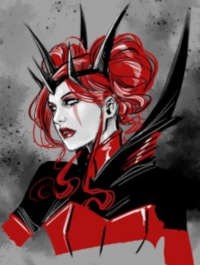
\includegraphics[height=250pt]{_img/pnjs/ktath-atn-queen.png}
\end{figure}
\subsubsection{Background}
Femme mystérieuse qui dirige la \textbf{Citadelle Hurlante} sur la planète Ktath’atn en l’an 0. Chaque année, elle organise une soirée durant laquelle elle reçoit de nombreux civils venus lui présenter des formes de vie organiques "intéressantes". Celui qui présente la forme de vie la plus intéressante se voit alors accorder un veux par la reine.

\subsubsection{Traits}

Sa \textbf{Vig}ueur dépend depuis combient de temps elle s’est nourrir. 

\begin{itemtable}[ c c c c c ]
    \textbf{Agi} & \textbf{Int} & \textbf{\^Ame} & \textbf{For} & \textbf{Vig} \\
    d10           & d10         & d4             & d4           & d8           
\end{itemtable}
\begin{itemtable}[ l X ]
    \textbf{Allure}      & 6 \\
    \textbf{Compétences} & Intimidation d8, Persuasion d8, Réseaux d10, Combat d8 \\
    \textdb{Atouts}      & Commandement
\end{itemtable}

\subsubsection{Défense}
\begin{itemtable}[ c c ]
    \textbf{Parade}     & \textbf{Résistance} \\
    6                   & 6 
\end{itemtable}

\newpage
	\section{Bestiaire}

\subsection{Pilier de bar Horoxien} \label{sec:horoxian-barfly}
\begin{figure}[h!]
    \centering
    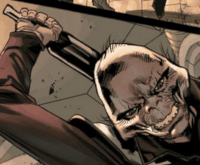
\includegraphics[height=200pt]{_img/bestiary/horoxian-barfly.png}
\end{figure}
\paragraph{Background}
Pas très malin, le pilier de bar horoxian se cache dans les cantina d’Horox III. Passe le plus clair de son temps à picoler et à refaire le monde avant de retourner à sa pauvre vie dénuée d’intérêt. C’est pourquoi dès que l’occasion se présente d’engager une bagarre, peu importe la raison, le pilier de bar Horoxien n’hésite pas \dots Bien bourré, le pilier de bar Horoxien ne sent pas la douleur, il n’est pas gêné par ses blessures.

\paragraph{Traits}

\begin{itemtable}[ c c c c c ]
    \textbf{Agi} & \textbf{Int} & \textbf{\^Ame} & \textbf{For} & \textbf{Vig} \\
    d4           & d4           & d4             & d8           & d8
\end{itemtable}
\begin{itemtable}[ l X ]
    \textbf{Allure}      & 6 \\
    \textbf{Compétences} & Combat d6
\end{itemtable}

\paragraph{Défense}
\begin{itemtable}[ c c ]
    \textbf{Parade}     & \textbf{Résistance} \\
    5 (-1 Alcool)       & 6
\end{itemtable}

\paragraph{Arme possible}
\begin{itemtable}[ X c c ]
    ~                & \textbf{Dégats} \\
    Bouteille cassée & 2d8
\end{itemtable}


\newpage

\subsection{Garde de la citadelle} \label{sec:citadel-guard}
\begin{figure}[h!]
    \centering
    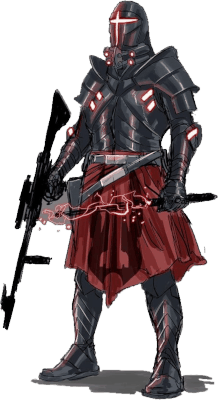
\includegraphics[height=200pt]{_img/bestiary/citadel-guard.png}
\end{figure}
\paragraph{Background}
Gardes au service de la reine. Ne parlent pas, ne réfléchissent pas et obéissent sans poser de questions aux ordres de \nameref{sec:bombinax}. Formés au combat depuis leur plus tendre enfance, les gardes de la citadelle sont équipés d’une armure lourde qui ne leur permet pas une grande liberté de mouvement mais leur confère une protection intégrale.

\paragraph{Traits}

\begin{itemtable}[ c c c c c ]
    \textbf{Agi} & \textbf{Int} & \textbf{\^Ame} & \textbf{For} & \textbf{Vig} \\
    d4           & d4           & d4             & d8           & d8
\end{itemtable}
\begin{itemtable}[ l X ]
    \textbf{Allure}      & 6 \\
    \textbf{Compétences} & Combat d10, Tir d8
\end{itemtable}

\paragraph{Défense}
\begin{itemtable}[ c c ]
    \textbf{Parade}     & \textbf{Résistance} \\
    7                   & 6 (+4)
\end{itemtable}

\paragraph{Arme possible}
\begin{itemtable}[ X c c ]
    ~                   & \textbf{Dégats} \\
    Fusil laser         & 2d8 + 2 \\
    Matraque neurale    & 1d6 + 1
\end{itemtable}

\newpage
\subsection{Symbiote Abersyn} \label{sec:symbiote-abersyn}
\begin{figure}[h]
    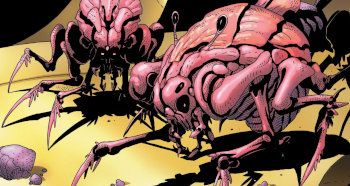
\includegraphics[width=\linewidth]{_img/bestiary/symbiote-abersyn.jpg}
\end{figure}

\subsubsection{Background}
Ces bestioles, grosses comme le poing sont bêtes et méchantes. Pas très dangereuses en soi mais si elles vous attrapent, elles s’immiscent en vous, viennent s’accrocher à votre cortex cérébral et prennent votre place aux commandes de votre corps. La bonne nouvelle est que vous ne mourrez pas, vous restez pleinement conscient de tout ce qu’il se passe sans pouvoir y faire quoi que ce soit.

\subsubsection{Combat}
Ces saletés n’ont pas de traits, elles ne sont pas jouées en combat comme des ennemis normaux. Elles n’apparaissent qu’en groupe, n’importe quelle attaque qui touche les explose. Par contre elles viennent perturber les combats.

Le MJ tire une carte pour tout le groupe de Symbiote. Quand c’est à leur tour de jouer, le MJ lance un dé (d2, d4, d6, \dots selon le nombre de créature présentent). Le résultat indique combien de joueurs sont attaqués par l’une de ces créatures. Elles attaquent avec \textbf{d6} à opposer à la \textbf{Par}ade de l’adversaire. Si l’adversaire ne pare pas, il n’y a pas de dégâts mais celui-ci, à son tour, doit réussir un jet de \textbf{Bag}arre pour se débarrasser du symbiote avant de pouvoir attaquer une cible différente. Il y passera son action tant qu’il ne réussit pas.
    \include{tex/armory}

	\onecolumn
	\nocite{*}
	\printbibliography
\end{document}